% Introduction

\chapter{Introduction}
\label{sec:sec_introduction}
Embedded systems are specialized computer systems that are designed to perform
specific tasks or functions within a larger system\cite{muench2018you}.They are
integral to a wide variety of devices and applications, enabling seamless
functionality and efficiency in our daily lives. These systems tightly
integrate hardware and software components to optimize performance, power
consumption, and system size\cite{eisele2022embedded}. The importance of
embedded systems lies in their ubiquity and versatility. They can be found in
numerous devices and industries, including consumer electronics\cite{andrae2010life},
telecommunications\cite{paulin1995dsp}, automotive\cite{Automoti68:online},
aerospace\cite{bieber2012security}, medical\cite{jafari2007medical}, and industrial
automation\cite{thramboulidis2007soa}. Examples of embedded systems include
microcontrollers\cite{gridling2007introduction} in smart home appliances\cite{kang2017enhanced},
digital signal processors in wireless communication devices\cite{kostic1997digital},
control systems in autonomous vehicles\cite{kostic1997digital}, and sensor
networks for monitoring and automation\cite{marwedel2021embedded}.

As the world becomes increasingly interconnected and reliant on technology,
the role of embedded systems continues to expand. They are essential for
enabling the \gls{iot}, as well as advancements in artificial intelligence,
robotics, medical instruments, and smart cities\cite{camposano1996embedded:ARTICLE}.
As of February 2023, there are an estimated 21.5 billion interconnected devices
in the world, according to Statistas\cite{IoTconne16:online}\cite{HowManyI1:online}.
This number is expected to continue to increase as internet consumption rises and
new gadgets and machinery are introduced to the market and by 2025,
it is projected that 75.44 billion \acrshort{iot} devices will be
installed worldwide\cite{HowManyI1:online}.

The number of embedded devices per person is significantly higher in developed
countries than in developing nations. For example, in the United States, there
were approximately 13 \acrshort{iot} devices per person in 2020\cite{Stateoft48:online}.
In comparison, the global average was around 3.5 \acrshort{iot} devices per person during
the same year\cite{CiscoAnn1:online}. In developed countries, prevalent devices
typically include intelligent home appliances\cite{wang2015anycontrol},
wearable technology\cite{poongodi2020wearable}, and
interconnected vehicles\cite{priyan2019survey}\cite{Internet36:online}.
Whereas, a greater concentration of devices aimed at supporting agriculture\cite{baranwal2016development},
healthcare\cite{pradhan2021iot}, and monitoring critical infrastructure in developing countries\cite{patil2012internet}.

The exponential growth of embedded systems necessitates robust security,
reliability, and efficiency measures to ensure the safety and functionality of
the technology we rely on daily\cite{muench2018you}. Mirai malware attacks have
demonstrated their potential for large-scale disruption, targeting devices like
routers, cameras, and DVRs to execute \gls{ddos} attacks\cite{KrebsOnS42:online}\cite{antonakakis2017understanding}.
In 2016, a \acrshort{ddos} attack on Dyn\cite{LargeDDo94:online}, a DNS provider, significantly
hindered user access to prominent services such as Twitter, Amazon, Tumblr, Reddit, Spotify, and
Netflix\cite{muench2018you}\cite{lindqvist2017future}. \textit{Ripple20},
a set of 19 critical vulnerabilities in Treck TCP/IP library\cite{TreckTCP63:online},
impacted IoT devices used in industrial control systems, healthcare devices,
and home appliances. URGENT/11\cite{WhatisUR60:online} and BadAlloc\cite{IoTriddl27:online},
discovered in the VxWorks \gls{rtos}\cite{VxWorksI53:online},
affected millions of embedded devices, including medical devices, industrial control systems,
and routers\cite{seri2019critical}. These vulnerabilities originate from memory
allocation functions and can lead to remote code execution, allowing attackers
to seize control of compromised devices\cite{1NewMess42:online}.

As the data breaches have become a prevalent issue in the digital age,
impacting individuals, businesses, and even governments\cite{10oftheB31:online}.
The following table:\ref{tab:data_breaches} highlights some of the most
significant data breaches that have occurred in
the 21st century\cite{The15big77:online}\cite{10oftheB31:online}.
These incidents serve as a reminder of the importance of robust
cybersecurity measures and the ongoing need for vigilance in
protecting sensitive information.

\begin{table}[ht]
\caption{Data Breaches in the 21st Century}
\label{tab:data_breaches}
\begin{tabularx}{\textwidth}{|l|X|}
\hline
\textbf{Company} & \textbf{Description} \\
\hline
Yahoo & In 2013 and 2014, Yahoo experienced two massive data breaches that affected approximately 3 billion user accounts. The breaches exposed users' personal information, including names, email addresses, and hashed passwords. \\
\hline
Equifax & In 2017, Equifax, one of the largest credit reporting agencies, suffered a breach that compromised the personal data of approximately 147 million Americans. The breach exposed sensitive information such as Social Security numbers, birth dates, and addresses. \\
\hline
Marriott International & In 2018, Marriott disclosed a data breach affecting approximately 500 million customers. The breach involved unauthorized access to the Starwood guest reservation database, exposing personal details, passport numbers, and payment card information. \\
\hline
Capital One & In 2019, a hacker gained access to Capital One's systems, resulting in the exposure of personal information of approximately 106 million individuals in the United States and Canada. The breach included names, addresses, credit scores, and Social Security numbers. \\
\hline
Facebook/Cambridge Analytica & In 2018, it was revealed that the data analytics firm Cambridge Analytica harvested personal data from millions of Facebook users without their consent. The incident raised concerns about privacy and data protection on social media platforms. \\
\hline
Target & In 2013, Target experienced a breach that affected approximately 41 million customer payment card accounts. The attack exploited vulnerabilities in the company's payment system, resulting in the theft of credit and debit card information. \\
\hline
\end{tabularx}
\end{table}
%\clearpage

Software testing\cite{myers2011art} is a critical process in the development of embedded systems,
especially as the number of embedded and software-controlled devices continues
to increase. With this expansion comes a growing potential platform for
illicit activities\cite{broekman2003testing}. To mitigate the risks associated with these devices,
it is imperative to improve the quality and security of the software produced.
While traditional testing methods, such as manual\cite{itkonen2009testers} and automated testing\cite{asfaw2015benefits},
have been widely used, they have limitations in uncovering all potential
vulnerabilities and edge cases, particularly in the context of software security\cite{819971}.

The \gls{edge-cases} refer to scenarios or inputs that are at or beyond the outer limits or boundaries
of what is considered normal or typical. These edge cases explore the software's behavior when
it encounters extreme or uncommon conditions. By testing software with edge cases, including
inputs near the upper and lower limits, unusual values, or unexpected scenarios, developers
can uncover potential issues or unexpected behaviors that may not be evident
during regular testing\cite{deng2023large}\cite{cunningham2019software}\cite{koopman2016challenges}.


Fuzz testing, also known as fuzzing involves dynamically generating input data variations
based on valid inputs, enabling the exploration of edge cases and the detection of bugs that are not directly
related to functional requirements\cite{9787842}\cite{fowler2018fuzz}\cite{deng2023large}\cite{eisele2022embedded}.
A dynamic testing technique which feeds the random data to a program till it crashes\cite{felderer2016security}\cite{yun2022fuzzing}.
Despite its success in general software testing, fuzz testing has not been implemented in the case
in company as part of their development lifecycle.

This study embarks on a journey to examine the potential benefits and implications
associated with the incorporation of fuzz testing techniques into the development
lifecycle of a specific case company. Operating in the semiconductor sector,
this company specializes in embedded software development. Although it currently
utilizes traditional testing methods, such as manual and automated testing, it
has yet to explore and adopt fuzz testing within its development processes.
This gap in testing practices, amidst rising cyber threats, fuels the motivation
for this study.

This study aims to explore the potential benefits and implications of introducing
fuzz testing into this company's development lifecycle. The pivotal research
question is: ``Can the implementation of fuzz testing techniques significantly
strengthen the security and quality of embedded systems developed by the case
company?'' The importance of this question cannot be overstated given the
role of the company's systems across numerous critical applications and industries.

To answer this research question, the study will begin with a \gls{csa} of
the company's existing software testing practices. This \acrshort{csa} will provide a
comprehensive understanding of the current testing environment and highlight
potential areas that could benefit from fuzz testing.

Upon completion of the \acrshort{csa}, the study will proceed to a proof-of-concept case
study using popular fuzz testing tools AFL++\cite{257204} and
LibFuzzer\cite{libFuzze17:online}.
This step will assess the effectiveness and feasibility of fuzz testing within
the company's specific development environment.

The ultimate objective of this study is to underline the potential benefits of
integrating fuzz testing into the embedded software development lifecycle, thus
providing valuable insights and a clear strategy for how fuzz testing can be
utilized to enhance software quality and security. This study aims to serve as
a practical guideline for the case company and equip them with actionable
insights for incorporating fuzz testing into their software development process.

\section{Background}

The focus of this study is a company located in Helsinki, Finland that specializes in designing
and developing embedded secure silicon \acrlong{ip} solutions\cite{Whatisan76:online}.
These solutions find extensive application across a variety of domains, including:

\begin{itemize}
\item Key Management Solutions\cite{WhatisKe81:online} for securing key provisioning
      management\cite{WhatisPr3:online} services
\item Security Protocol Solutions\cite{TypesofS33:online} for safeguarding
      networking services\cite{kwon2014drives}
\item \gls{dpa} Solutions\cite{Differen58:online}\cite{SIDECHAN21:online} for
      protecting against side-channel attacks\cite{SIDECHAN21:online}\cite{standaert2010introduction}
\item Anti-Counterfeiting Products\cite{PuttingA14:online} and \gls{rot}\cite{WhatisRo39:online} products,
      which provide highly secure hardware\cite{WhatisHa66:online}, software, and firmware\cite{WhatIsFi49:online} components
\end{itemize}

The company holds an \acrlong{iso} 9001 standard\cite{ISOISO9044:online} certification.
This certification, internationally recognized for quality management,
underlines the company's dedication to continuous improvement,
a customer-centric approach, and top-level management engagement.
In the context of the company's practices, this translates to a
commitment to enhancing their system testing processes and standards, which in turn,
boosts the security and quality of its products.

In terms of software testing, the company utilizes an array of methodologies
including manual, integration, automation, and exploratory testing\cite{WhatisEx64:online}.
A significant emphasis is placed on security testing\cite{baker2013analyzing} to proactively
identify and mitigate potential vulnerabilities and risks. Furthermore,
the company implements \gls{ci/cd} practices,
facilitating incremental development, integration, and testing. This approach
allows for early error detection, efficient location of issues, and
ultimately enhances testing efficiency\cite{DevOpsin19:online}.

In the evolving landscape of automated security testing, fuzzing has
garnered substantial attention for its potential. With this in mind,
the company is evaluating various fuzzing tools and techniques for its
embedded products. The objective of this evaluation is to investigate the
potential enhancements in the quality and coverage of their existing
testing processes.

\section{Objectives, Purpose and Scope}

In the context of the rapidly growing technology landscape, the importance of
robust and efficient software testing methods cannot be overstated.
Embedded systems, being integral to countless applications and industries,
demand meticulous testing to ensure their reliability, functionality, and most
importantly, security. Traditional software testing methods, while effective to
an extent, may not be sufficient to uncover all vulnerabilities in these
complex systems. Therein lies the necessity for advanced testing techniques
such as fuzz testing, which are designed to thoroughly probe software and uncover
issues that could potentially be exploited, leading to system breakdowns or breaches.

Fuzz testing, or fuzzing, has shown remarkable potential in enhancing software
quality and security, and as a result, it has garnered significant interest
in the software testing field. Despite this, its application, particularly in
embedded systems, remains somewhat limited, largely due to the lack of
understanding and awareness about the technique.
\subsection{Objectives}
\begin{itemize}
\item Conduct a thorough analysis of the potential benefits and practical
      applications of fuzzing as an advanced software testing technique in the context of embedded systems.
\item Perform a comparative analysis of the leading fuzzing tools-AFL++ and libFuzzer,
      to determine the tool best suited to the company's specific needs.
\item Carry out a proof-of-concept case study using the chosen fuzzing tool to
      evaluate its ability to uncover software vulnerabilities and improve system security and quality.
\item Prepare guidelines for future integration of the chosen fuzzing tool
     into the company's existing \acrshort{ci/cd} practices.
\end{itemize}

\subsection{Purpose}
\begin{itemize}
\item Highlight the limitations of traditional software testing methods for
      embedded systems and emphasize the necessity for more advanced techniques like fuzzing.
\item Demonstrate how fuzzing can augment software quality and security by
      uncovering vulnerabilities that may be missed by conventional testing methods.
\item Support the case company's goal of enhancing its software testing practices by
      introducing a well-suited fuzzing tool into its development cycle.
\end{itemize}
\subsection{Scope}
This study will focus on the evaluation and application of fuzzing as a software
testing technique for embedded systems, within the specific context of the
case company. The research will involve a comparative analysis of three leading
fuzzing tools—AFL++, libFuzzer, and Atheris—and will include a proof-of-concept
case study. Additionally, while this study will provide guidelines for
integrating the chosen fuzzing tool into CI/CD practices,
it will not cover the actual implementation or assessment of these practices.
\clearpage

\section{Structure of the Thesis}
% \begin{figure}[ht]
%         \centering
%         \AltText{Thesis Flow Chart}{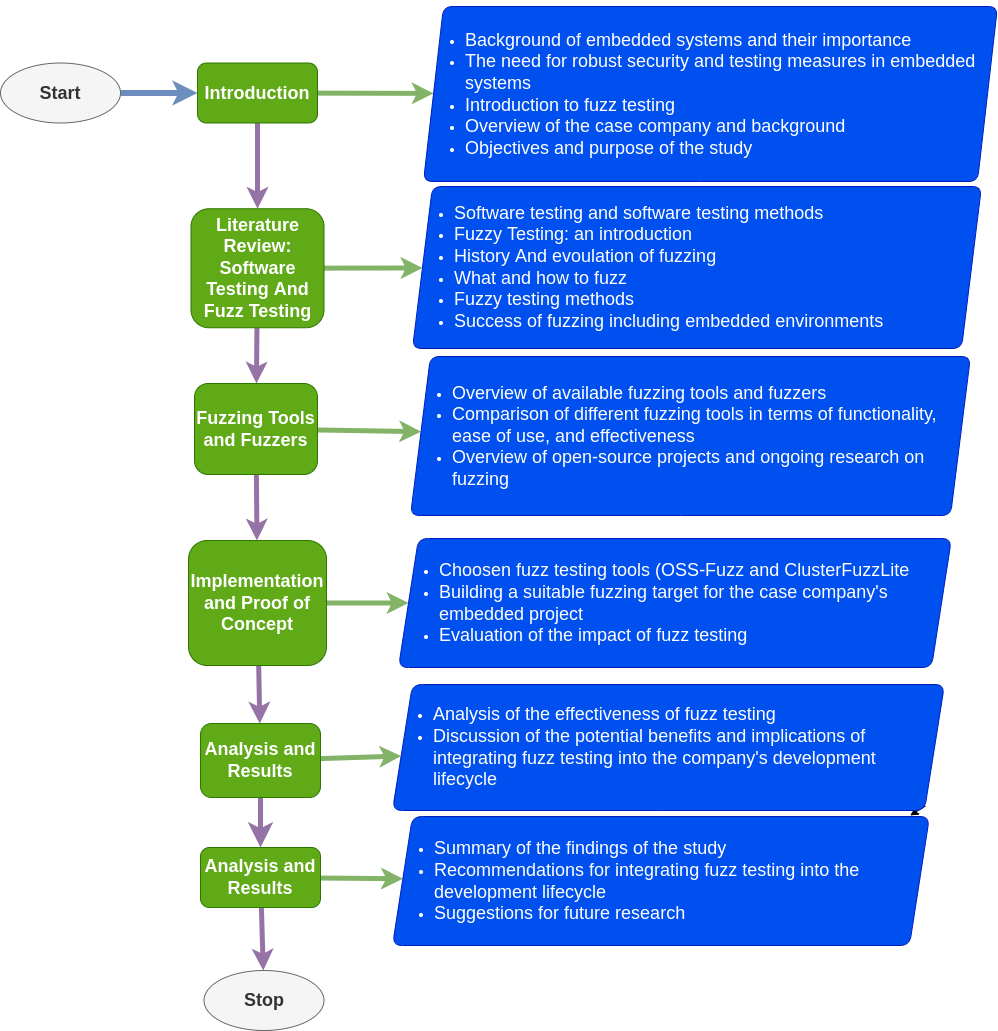
\includegraphics[width=14.5cm,height=20.4cm,keepaspectratio]{thesis_structure}}
%         \caption{Thesis Flow Chart}\label{fig:thesis_structure}
% \end{figure}

\begin{figure}[h]
      \centering
      \adjustbox{width=\textwidth}{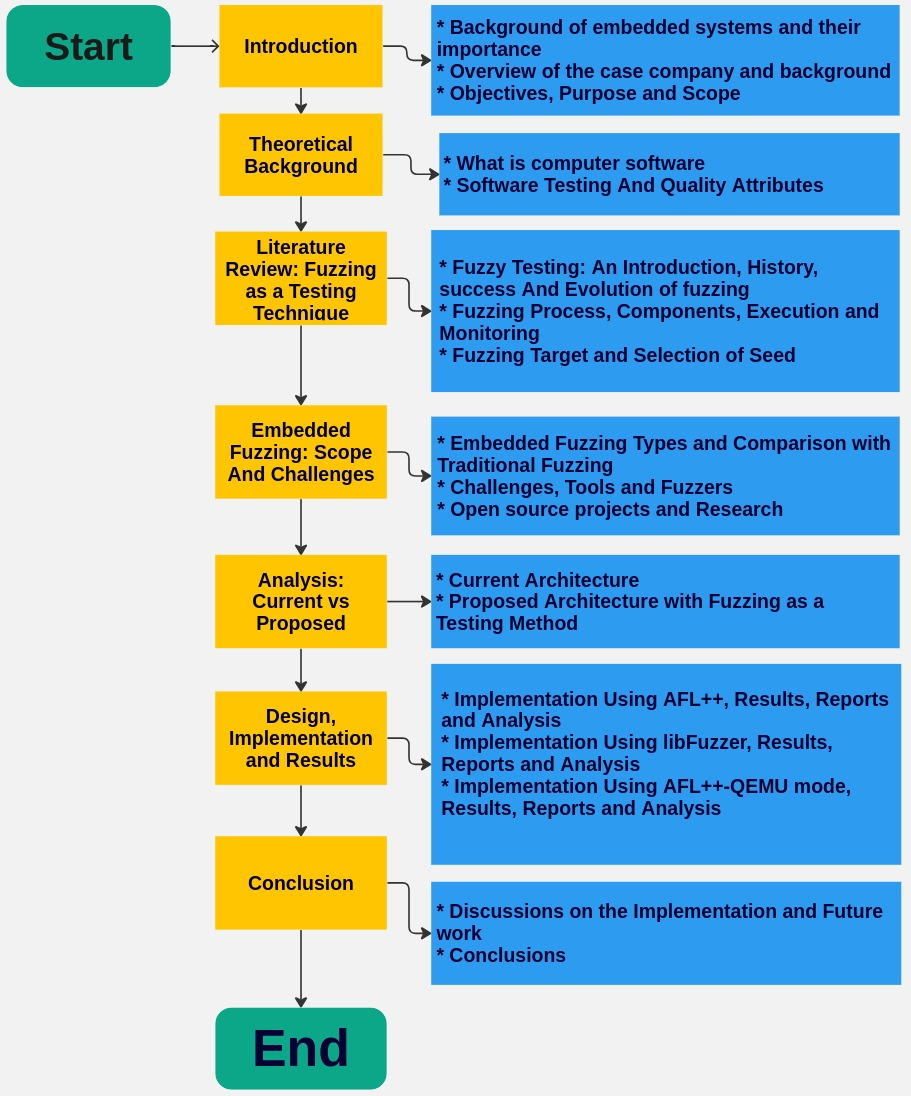
\includegraphics{thes_str.png}}
      \caption{Thesis Flow Chart}\label{fig:thes_str.png}
\end{figure}

\clearpage